\section{Conditional expectations for the full 2021 sample}
\label{sec:v505-projections}
The released 10\% sample provides a way to ask what the full-sample fit might
look like if one of its local excesses persists. Studies v5.6.0 and v5.6.1
make this assumption explicit: they inject one resolution-shaped peak at a
time into a continuum fitted to the released sample, increase the exposure
by ten and repeat the moving-window analysis. The exercise predicts both a
central excess and its effect on nearby background fits. It uses no observed
full-2021 spectrum.

\subsection{Exposure scaling and the injection strength}
For unchanged selection, signal shape and background composition, an excess
dominated by counting statistics would approximately obey
\begin{equation}
 S_{100}=kS_f,\qquad B_{100}=kB_f,\qquad
 Z_{100}\simeq\frac{kS_f}{\sqrt{kB_f}}=\sqrt{k}\,Z_f,
 \qquad k=1/f.
 \label{eq:v505-scaling}
\end{equation}
Thus $Z_{100}^{\rm target}=\sqrt{10}\,Z_{10\%}$ for the released sample.
This is a conditional persistence estimate, not a maximum possible or most
probable future significance. The regions were selected after inspecting
partial data, and a fluctuation need not grow as a real signal would.
A global probability would also require the mass search and the selection
of these hypotheses to be accounted for.

For independent Poisson bins with known background, the corresponding
Asimov relation is exact under a common exposure rescaling:
\begin{align}
 Z_{A,\mathrm{known}\ b}^2(s,b)
 &=2\sum_i\left[(s_i+b_i)\log\left(1+\frac{s_i}{b_i}\right)-s_i\right],\\
 Z_{A,\mathrm{known}\ b}(ks,kb)&=\sqrt{k}\,Z_{A,\mathrm{known}\ b}(s,b).
\end{align}
This identity does not require $s_i\ll b_i$. It does require the background
to be known; the learned and profiled GP background need not obey it.

The saved study compares two amplitudes. Direct yield scaling gives
$A_{\rm yield}=k\max(\widehat A_f,0)$. The second amplitude, $A_{\rm match}$,
is adjusted to satisfy
\begin{equation}
 Z_A^{\rm GP}(A_{\rm match};m_0)=\sqrt{k}Z_f,\qquad
 R_A=A_{\rm match}/A_{\rm yield}.
\end{equation} The matched spectrum is deterministic,
$n_i^A=b_i+A_{\rm match}t_i$, and each toy is an independent Poisson draw
from that expectation. Because the GP is conditioned again for each
spectrum and tested mass, direct yield scaling need not reproduce the
simple significance rule. Agreement of the matched injection with the
rule is imposed during construction.

\begin{table}[H]\centering\small
\begin{tabular}{rrrrr}\toprule
$m_0$ [MeV] & $Z_f$ & $\sqrt{k}Z_f$ & Yield-scaled $Z_A$ & Toy $Z$ median [16,84\%]\\\midrule
65 & 2.40 & 7.58 & 6.76 & 7.63 [6.10, 8.47] \\
78 & 2.81 & 8.88 & 8.39 & 8.64 [7.80, 10.18] \\
93 & 1.51 & 4.77 & 4.45 & 4.63 [3.92, 5.58] \\
123 & 1.18 & 3.74 & 3.64 & 3.51 [2.89, 4.63] \\
160 & 1.49 & 4.71 & 4.54 & 4.39 [3.50, 5.71] \\
208 & 1.41 & 4.46 & 4.16 & 4.23 [3.41, 5.30] \\
\bottomrule\end{tabular}
\caption{Source local scores, exposure-scaling targets, direct yield-scaled
Asimov scores and the fixed-mass scores of 20 target-matched Poisson toys per
scenario. Quantiles describe this small conditional ensemble.}
\label{tab:v505-ten}\end{table}
The largest target among these six regions is $8.88$ at 78 MeV, followed by
$7.58$ at 65 MeV. Their saved toy medians are $8.64$ and $7.63$, respectively.
The region called ``120 MeV'' in the meeting slides is injected at 123 MeV
in the numerical catalogue. The table uses those actual masses and separates
the target from the toy median throughout. The remaining targets are about
$3.7$--$4.8$; none is a forecast of calibrated discovery significance.

\subsection{The meaning of a maximum in the toy catalogue}
The largest fixed-mass score among the 20 saved 78 MeV toys is 11.62, whereas
their median is 8.64. A finite-ensemble maximum is expected to exceed a
typical realization and depends on how many toys are drawn. For independent
fixed-mass scores with cumulative distribution $F$, the maximum satisfies
\begin{equation}
 \Pr(M_{20}\leq z)=F(z)^{20}.
\end{equation}
Under the additional illustrative assumption $Z\sim N(Z_A,1)$, its median
would be $Z_A+\Phi^{-1}(2^{-1/20})\simeq Z_A+1.82$. This normal model has
not been validated for these GP fits. A maximum over nearby tested masses
is yet another statistic and depends on their correlations. Neither maximum
is an upper bound on the significance that future data can produce.

\subsection{Nearby fitted deficits and upper-limit structure}
A peak can affect hypotheses outside its own fit window. As the excluded
window moves, some injected counts enter the training sidebands. The GP
then predicts a higher continuum inside a nearby window, which can produce
a negative fitted signal and a tighter upper limit. The signed profile score
retains this response:
\begin{equation}
 r(m)=\operatorname{sign}(\widehat A)
 \sqrt{2[\ell(\widehat A,\widehat\theta)-\ell(0,\widehat\theta_0)]},
 \qquad Z_0(m)=\max(0,r(m)).
\end{equation}
These negative structures are called echoes in the standalone study.
Their width and position depend on the background, resolution and training
exclusion, as illustrated in Figure~\ref{fig:v505-ten-summary}.

At each mass, v5.6.1 profiles the GP-constrained Poisson likelihood
\begin{equation}
 \ell(A,\theta;m)=\sum_i[n_i\log\lambda_i-\lambda_i]
 -\tfrac12\theta^T\theta,\qquad
 \lambda_i=b_i+(L\theta)_i+A\,t_i(m),\quad LL^T=C_b.
\end{equation}
The bounded asymptotic construction gives $A_{90}$ from
$\mathrm{CL}_s(A_{90})=0.10$. To compare the injected and continuum-only
Asimov spectra, the echo calculation uses
\begin{equation}
 R(m)=\frac{A_{90}^{\rm injected}(m)}{A_{90}^{(b)}(m)},\qquad
 D=1-R(m_e),\qquad m_e\in m_0\pm[2,8]\sigma_m(m_0).
 \label{eq:v505-echo}
\end{equation}
The deepest local minimum on each saved flank is selected, with a flank
minimum used when no interior minimum exists. Flanks are clipped to the
scan support. The connected saved-grid interval with $R\leq0.90$ records
the extent of a depression of at least 10\%. These choices precede any
inspection of the full-data spectrum.

\begin{figure}[p]\centering
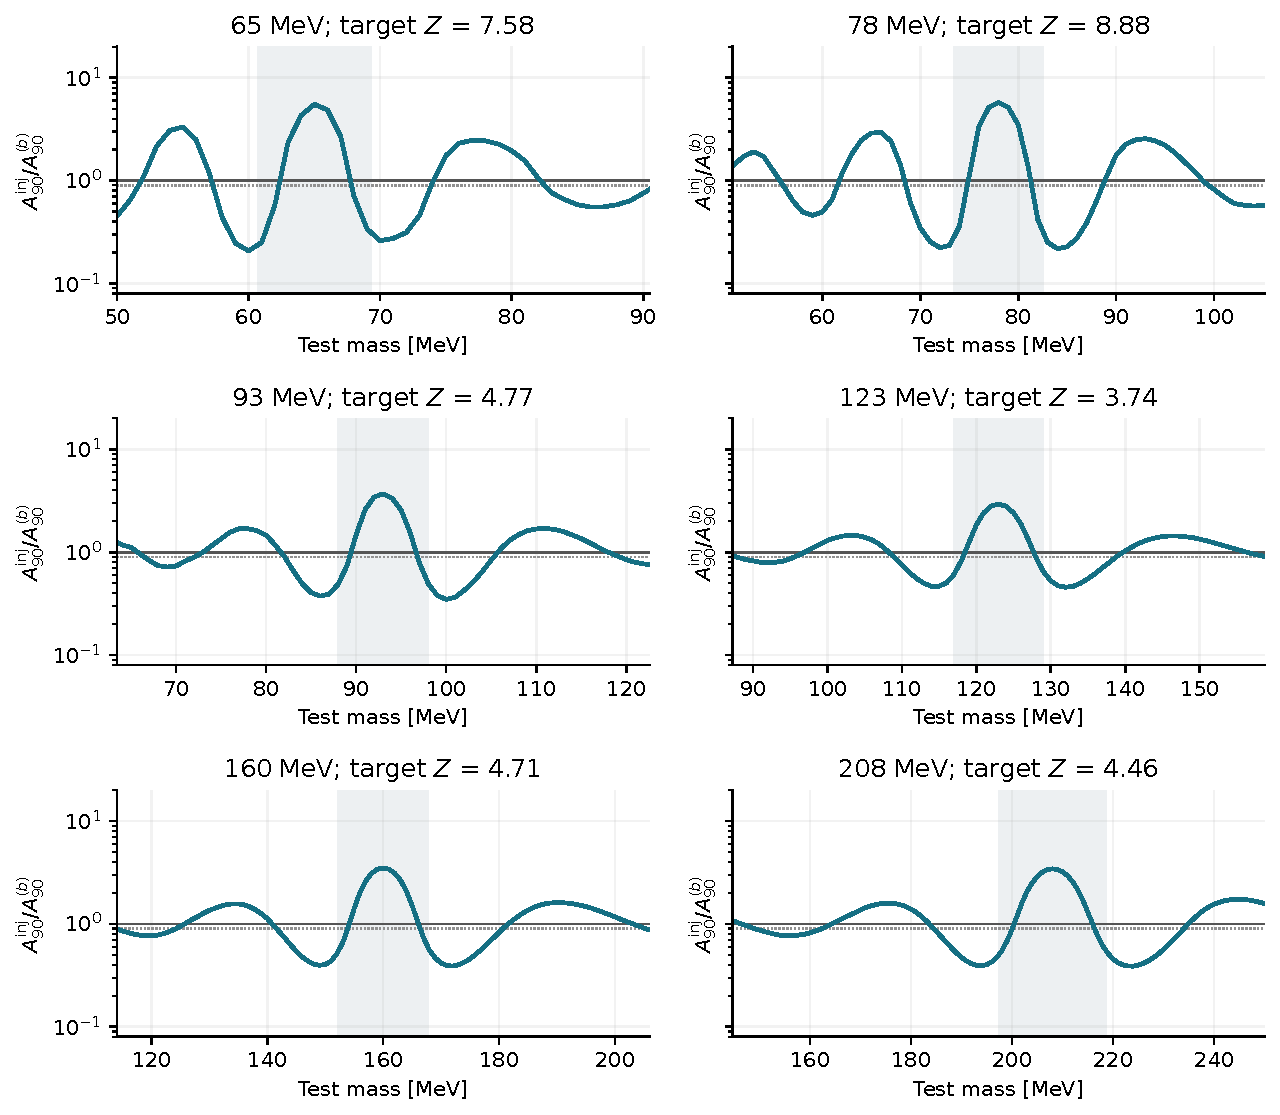
\includegraphics[width=\linewidth]{../figures/v505_ten_echo_summary.pdf}
\caption{Six alternative injections based on the 10\% sample. Curves show
the matched-Asimov count-limit ratio in Eq.~\eqref{eq:v505-echo}; shaded
central intervals mark $|m-m_0|<2\sigma_m$, outside the echo search.
Each panel uses its own fitted continuum. The alternatives are not a
simultaneous six-peak hypothesis.}\label{fig:v505-ten-summary}\end{figure}

For a 65 MeV injection, the selected Asimov minima occur at 60 and 70 MeV,
with count-limit reductions of 79.2\% and 74.0\%. Both lie at a declared
flank boundary. For the 78 MeV injection the minima occur at 72 and 84 MeV,
with reductions of 77.7\% and 78.2\%. The saved mass grid is 1 MeV, so these
positions should not be read with finer precision.

The coupling plots convert count limits using the prompt density of each
spectrum, whereas $R$ keeps the normalization common:
\begin{equation}
 K_n(m)=\frac{3\pi m f_{\rm rad}^{\rm eff}}{2\alpha}\rho_n(m),\qquad
 \eps^2_{90,n}(m)=\frac{A_{90,n}(m)}{K_n(m)}B_e^{-1}(m).
\end{equation}
Here $f_{\rm rad}^{\rm eff}=0.0477$ and $\rho_n$ uses fractional-bin overlap
within $\pm1.64\sigma_m$, with mass and density in consistent units.
The visible branching correction is one below the dimuon threshold and
$B_e^{-1}=1+\sqrt{1-4u}(1+2u)$ above it, where $u=(m_\mu/m)^2$.
The limit of the matched-Asimov spectrum is not generally the mean or median
of the toy limits, because conditioning, profiling and finding the limit
are nonlinear operations.

\subsection{What the catalogue can test}
The catalogue provides concrete patterns to compare with a future spectrum:
the signal-shaped excess, its fitted amplitude, and the associated changes
in nearby limits. Agreement in one panel would not validate the generating
background or identify a particle. Real structures can have different
shapes, and several nearby features can interfere through the background
fit. Twenty toys per scenario suffice to illustrate these responses, but do
not determine rare tails, global significance or the chance that a specified
echo will occur. Appendix~\ref{app:v505-one} gives the historical 1\%
projections and selected fit catalogues under their separate source assumptions.

\fig{1.0}{../figures/v561_ten_65.pdf}{The 65 MeV example from v5.6.1:
full-range coupling limits, count-limit ratios and signed profile scores.
All 20 saved toy curves are shown. Their spread describes repeated samples
from the specified injection, not a background-only expected band or a
coverage-calibrated interval.}{fig:v505-ten65}
\fig{1.0}{../figures/v561_ten_75.pdf}{The corresponding 78 MeV example.
A central excess can accompany lower upper limits on either side as its
counts enter neighboring GP training regions.}{fig:v505-ten78}
